\documentclass[12pt,a5]{bxjsarticle}

\usepackage{xltxtra}
\setmainfont{IPAPMincho}
\setsansfont{IPAPGothic}
\setmonofont{IPAGothic}
\XeTeXlinebreaklocale "ja"

\usepackage{hyperref}
\usepackage{listings}
\usepackage{verbatim}

\newcommand{\e}{\mathrm{e}}

\title{物理学情報処理論2 problem7}
\date{}

\begin{document}
\maketitle

\section{}

\[
  V(x) = -3\mathrm{sech}^2(x), -\frac{d^2u}{dx^2} + V(x) u = E u
\]
の定常状態を求める。
Symplectic法では精度が不足していたため、4次のR-K法にて計算を行う。

$ E_{even} = -1.69722, E_{odd} = -0.091673 $ のようになった。
これらは解析的に求められた値、
$ E_0 = - \frac{1}{4}(\sqrt{13}-1)^2 \sim -1.6972, E_1 = - \frac{1}{4}(\sqrt{13}-3)^2 \sim -0.091673 $ と比較して相対誤差1\%以内におさまっている。

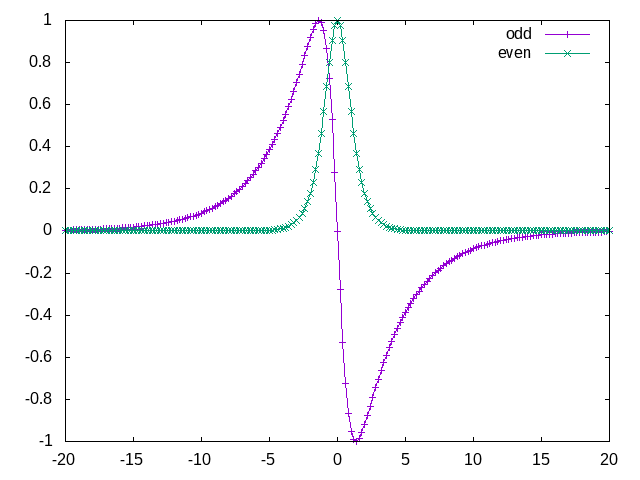
\includegraphics[width=\linewidth]{graph.png}

以下のスクリプトを用いて、orbit.datから図を生成した。
\lstinputlisting[caption=plot.sh,language=bash]{plot.sh}

\end{document}
